\documentclass[a4paper, 11pt]{article}
\usepackage[margin=20mm]{geometry}
\usepackage{lmodern}
\usepackage{multicol}
\usepackage{titlesec}
\usepackage{graphicx}
\usepackage{caption}
\usepackage{booktabs}
\usepackage{amsmath}
\usepackage{microtype}
\usepackage{url}
\graphicspath{{figures/}{../analysis/results/}}

\newcommand\textline[4][t]{%
  \par\smallskip\noindent\parbox[#1]{.333\textwidth}{\raggedright #2}%
  \parbox[#1]{.333\textwidth}{\centering #3}%
  \parbox[#1]{.333\textwidth}{\raggedleft #4}\par\smallskip%
}

\titleformat{\section}{\normalfont\bfseries}{\thesection.}{0.6em}{}
\titleformat{\subsection}{\normalfont\bfseries\small}{\thesubsection.}{0.6em}{}
\titlespacing{\section}{0pt}{4pt}{2pt}
\setlength{\abovedisplayskip}{3pt}
\setlength{\columnsep}{6mm}
\captionsetup{font=scriptsize, skip=2pt}
\linespread{0.95}\selectfont
\newenvironment{tightcenter}{\par\nobreak\vskip 2pt\centering}{\par\vskip 2pt}
\renewcommand{\arraystretch}{0.95}

\begin{document}
\pagestyle{empty}

\textline[t]{\,\,}{Preprint of graduation study}{Jul. 28, 2026}
\vspace{0.1\baselineskip}
\begin{flushright}
  \begin{tabular}{@{}ll@{}}
    Name:       & Adriel Imaran Santoso  \\
    Supervisor: & Prof. Koichi Hashimoto \\
  \end{tabular}
\end{flushright}
\begin{center}
  Title: Tactile-Feedback Teleoperation: Grip Force and Grasping Performance \\
  Across Haptic Actuator Types for Fragile and Deformable Objects
\end{center}
\vspace{0.2\baselineskip}
\begin{multicols}{2}

  \section{Introduction}

  When we pick up an egg, our fingers let us know how hard we are squeezing, so we stop
  before it cracks. In \emph{teleoperation}, where a user controls a robot remotely, that sense
  is missing, and the user can only guess whether the grip is too loose to hold the object or
  firm enough to break it.

  The common solution is a wearable \emph{haptic actuator}, a device that reproduces that sense via
  vibrations or forces applied to the skin (Patel et al., 2025), but research comparing different
  actuators is limited, with most studies instead asking whether feedback improves performance over
  no feedback at all (Thomas et al., 2019). We tackle both questions at once: does touch feedback help users grasp specific types of
  objects, and does it matter which actuator delivers that feedback?

  \section{System}

  \begin{tightcenter}
    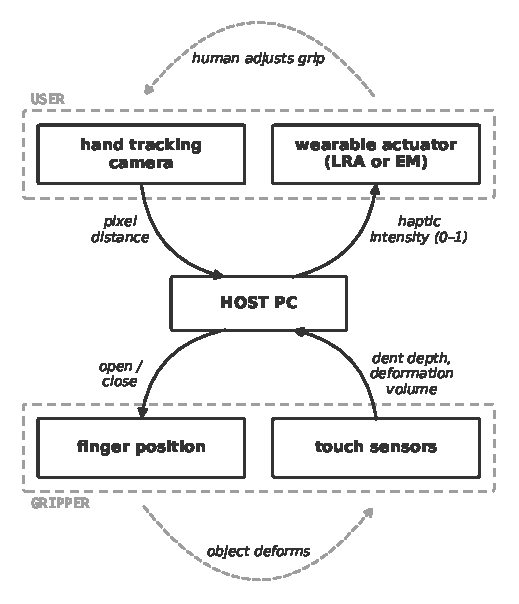
\includegraphics[width=0.95\columnwidth]{preprint_fig1.eps}
    \captionof{figure}{Signal flow of the experimental setup. The PC translates pixel distance
      between the thumb and index finger into gripper position command, and touch sensor data into
      a normalized intensity value between $0$ and $1$.}
    \label{fig:signalflow}
  \end{tightcenter}

  The system setup is detailed in Figs.~\ref{fig:signalflow} and \ref{fig:hardware}. Two actuator types
  are compared in this study: a \emph{linear resonant actuator (LRA)}, a small motor that vibrates
  along one axis, like the kind used in smartphones (Pacchierotti et al., 2017), and an
  \emph{electromagnetic actuator (EM)} adapted from (Vechev et al., 2019). Where each actuator
  sits was simply carried over from earlier work.

  \begin{tightcenter}
    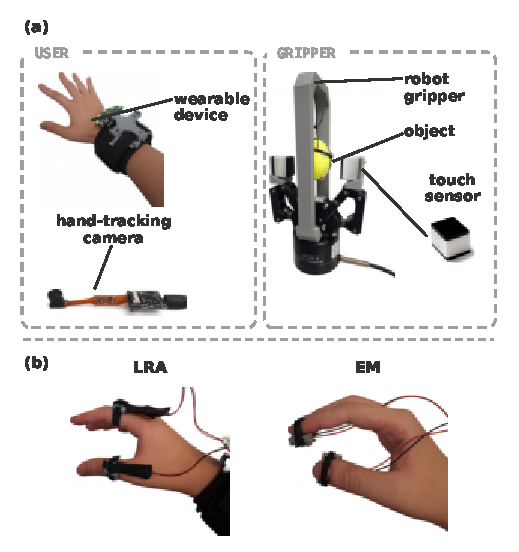
\includegraphics[width=0.95\columnwidth]{preprint_fig2.eps}
    \captionof{figure}{Hardware components of the experimental setup. (a) User and gripper
      apparatus as grouped in Fig.~\ref{fig:signalflow}. (b) LRA and EM actuator type connected
      to the wearable device.}
    \label{fig:hardware}
  \end{tightcenter}

  \section{Method}

  \begin{tightcenter}
    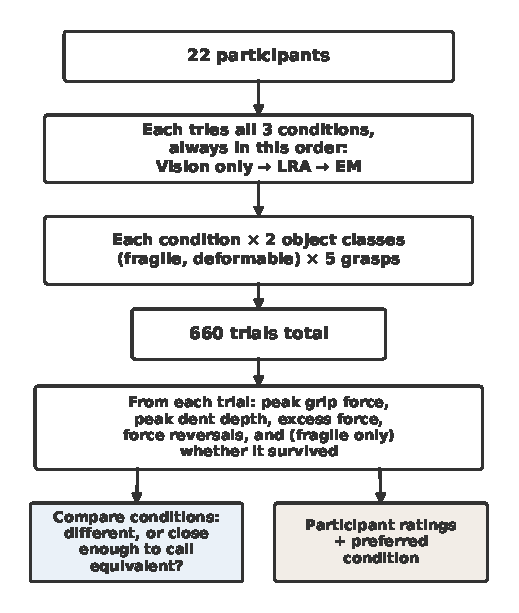
\includegraphics[width=0.95\columnwidth]{preprint_fig3.eps}
    \captionof{figure}{The experiment, start to finish.}
    \label{fig:methodflow}
  \end{tightcenter}

  Participants grasped two classes of object: \emph{fragile} ones, which break suddenly when
  squeezed too hard, and \emph{deformable} ones, which instead change shape gradually.
  Fig.~\ref{fig:methodflow} walks through the experiment: what each participant did, how many
  trials that produced, what we measured from each one, and how we compared conditions
  afterward. ``Excess force'' means squeezing that continued after the dent had already
  stopped getting deeper, wasted effort since intensity depends only on depth, not force.

  \section{Results}

  \begin{tightcenter}
    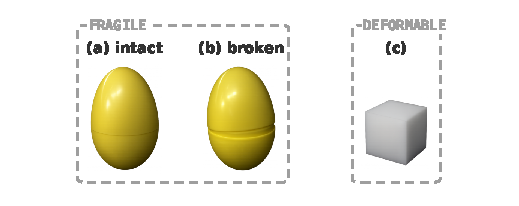
\includegraphics[width=0.95\columnwidth]{preprint_fig4.eps}
    \captionof{figure}{Fragile objects. (a) How often the object survived, 110 trials per
      condition. (b) Excess force per participant (log scale, $+1$).}
    \label{fig:results}
  \end{tightcenter}

  Touch feedback clearly helped with fragile objects (Fig.~\ref{fig:results},
  Table~\ref{tab:quant}). With feedback, people stopped over-squeezing almost immediately:
  excess force dropped roughly ninefold with the LRA and sixfold with the EM, and they needed
  much less trial-and-error to find the right grip, from a median of 7 reversals down to 5 and
  2. That translated into fewer breakages, too, with survival rising from 62\% under vision
  alone to 81\% and 78\% with the two actuators. Deformable objects told a different story:
  since they barely dent the gel and never break outright, feedback made no reliable
  difference there. Participants felt the benefit as well, rating both haptic conditions far
  above vision only, especially for feeling how hard they were gripping and for confidence in
  the grasp (Fig.~\ref{fig:likert}a); asked to pick a favorite, 17 of 22 chose the LRA, though
  no single measure could tell the two actuators apart (Fig.~\ref{fig:likert}b).

  \begin{tightcenter}
    \begin{minipage}{\columnwidth}
      \captionof{table}{Typical (median) values on fragile objects, $N=22$. V = vision only.
        Survival rate and force reversals were the most reliable improvements; peak dent depth
        is capped by the 1.0~mm safety cutoff.}
      \label{tab:quant}
      \scriptsize
      \centering
      \begin{tabular}{@{}lrrr@{}}
        \toprule
        Metric                 & V     & LRA   & EM    \\
        \midrule
        Peak grip force (a.u.) & 20100 & 12300 & 16000 \\
        Excess force (a.u.)    & 1530  & 170   & 260   \\
        Force reversals (\#)   & 7.0   & 5.0   & 2.0   \\
        Survival rate          & 0.60  & 0.80  & 0.90  \\
        Peak dent depth (mm)   & 0.98  & 0.95  & 0.98  \\
        \bottomrule
      \end{tabular}
    \end{minipage}
  \end{tightcenter}

  \begin{tightcenter}
    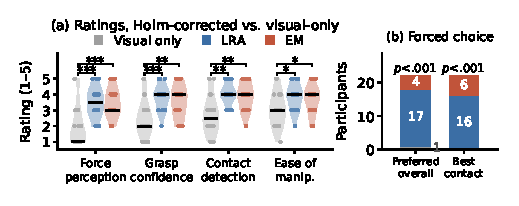
\includegraphics[width=0.95\columnwidth]{preprint_fig5.eps}
    \captionof{figure}{Participant ratings ($n=22$). (a) Ratings per item (spread, individual
      points, median) compared against vision only; stars mark differences judged
      statistically reliable. (b) Which condition was preferred.}
    \label{fig:likert}
  \end{tightcenter}

  \section{Discussion}

  The main limitations are the fixed trial order, which may have introduced practice or
  fatigue effects; the confound between the two actuators, which differ in technology,
  mounting position, and how well hand tracking worked, so any preference between them may
  reflect smoother control rather than a better sensation; 2D and uncalibrated hand tracking;
  grip force measured as a proxy rather than in newtons; and an end-to-end delay that still
  needs a bench measurement. Future work will balance the order, mount both actuators in the
  same place, calibrate against a load cell, and send a spatial feedback pattern rather than
  one number per finger.

  \section{Conclusion}

  Tactile feedback made grasping fragile objects safer, while a larger, better-controlled
  study is needed to tell the two actuators apart.

  \section{References}

  \begin{scriptsize}
    \noindent\hangindent=1em Patel, S., Rao, Z., Yang, M., \& Yu, C. (2025). Wearable haptic
    feedback interfaces for augmenting human touch. \textit{Advanced Functional Materials},
    \textit{35}(4), 2417906. \url{https://doi.org/10.1002/adfm.202417906}

    \noindent\hangindent=1em Thomas, N., Ung, G., McGarvey, C., \& Brown, J. D. (2019).
    Comparison of vibrotactile and joint-torque feedback in a myoelectric upper-limb
    prosthesis. \textit{Journal of NeuroEngineering and Rehabilitation},
    \textit{16}(1), 73. \url{https://doi.org/10.1186/s12984-019-0545-5}

    \noindent\hangindent=1em Johansson, R. S., \& Flanagan, J. R. (2009). Coding and use of
    tactile signals from the fingertips in object manipulation tasks. \textit{Nature Reviews
      Neuroscience, 10}(5), 345--359.

    \noindent\hangindent=1em Lin, C., Zhang, H., Xu, J., Wu, L., \& Xu, H. (2023). 9DTact: A
    compact vision-based tactile sensor for accurate 3D shape reconstruction and generalizable
    6D force estimation. \textit{arXiv preprint arXiv:2308.14277}.

    \noindent\hangindent=1em Pacchierotti, C., Sinclair, S., Solazzi, M., Frisoli, A.,
    Hayward, V., \& Prattichizzo, D. (2017). Wearable haptic systems for the fingertip and the
    hand: Taxonomy, review, and perspectives. \textit{IEEE Transactions on Haptics, 10}(4),
    580--600.

    \noindent\hangindent=1em Vechev, V., Zarate, J. J., Lindlbauer, D., Hinchet, R., Shea, H.,
    \& Hilliges, O. (2019). TacTiles: Dual-mode low-power electromagnetic actuators for
    rendering continuous contact and spatial haptic patterns in VR. \textit{2019 IEEE
      Conference on Virtual Reality and 3D User Interfaces (VR)}, 312--320.

  \end{scriptsize}

\end{multicols}

\end{document}
